%---------------------------------------------------------------------------%
\lecture{Research Presentation}{lec_present_method}
%---------------------------------------------------------------------------%
\section{Theory}
%---------------------------------------------------------------------------%
\begin{frame}[fragile]
    \frametitle{Ridge Regression}
    Similar to OLS, ridge minimizes the sum of squared residuals (SSR), but includes an $\ell_2$-norm shrinkage penalty with a tuning parameter ($\lambda$):
    \begin{align}
    \label{eqn:eqn1}
    \underbrace{\sum_{i=1}^{n}\left(y_{i}-\beta_{0}-\sum_{j=1}^{p} \beta_{j} x_{i j}\right)^{2}}_\text{SSR} + \underbrace{\lambda\sum_{j=1}^{p}\beta_{j}^{2}.}_\text{shrinkage penalty}
    \end{align}
    \begin{itemize}
        \item If $\lambda=0$, we are left with the OLS estimates.
        \item As $\lambda$ increases, the estimated ridge coefficients shrink towards zero.
    \end{itemize}
\end{frame}
%---------------------------------------------------------------------------%
\begin{frame}[fragile]
    \begin{figure}[b]
        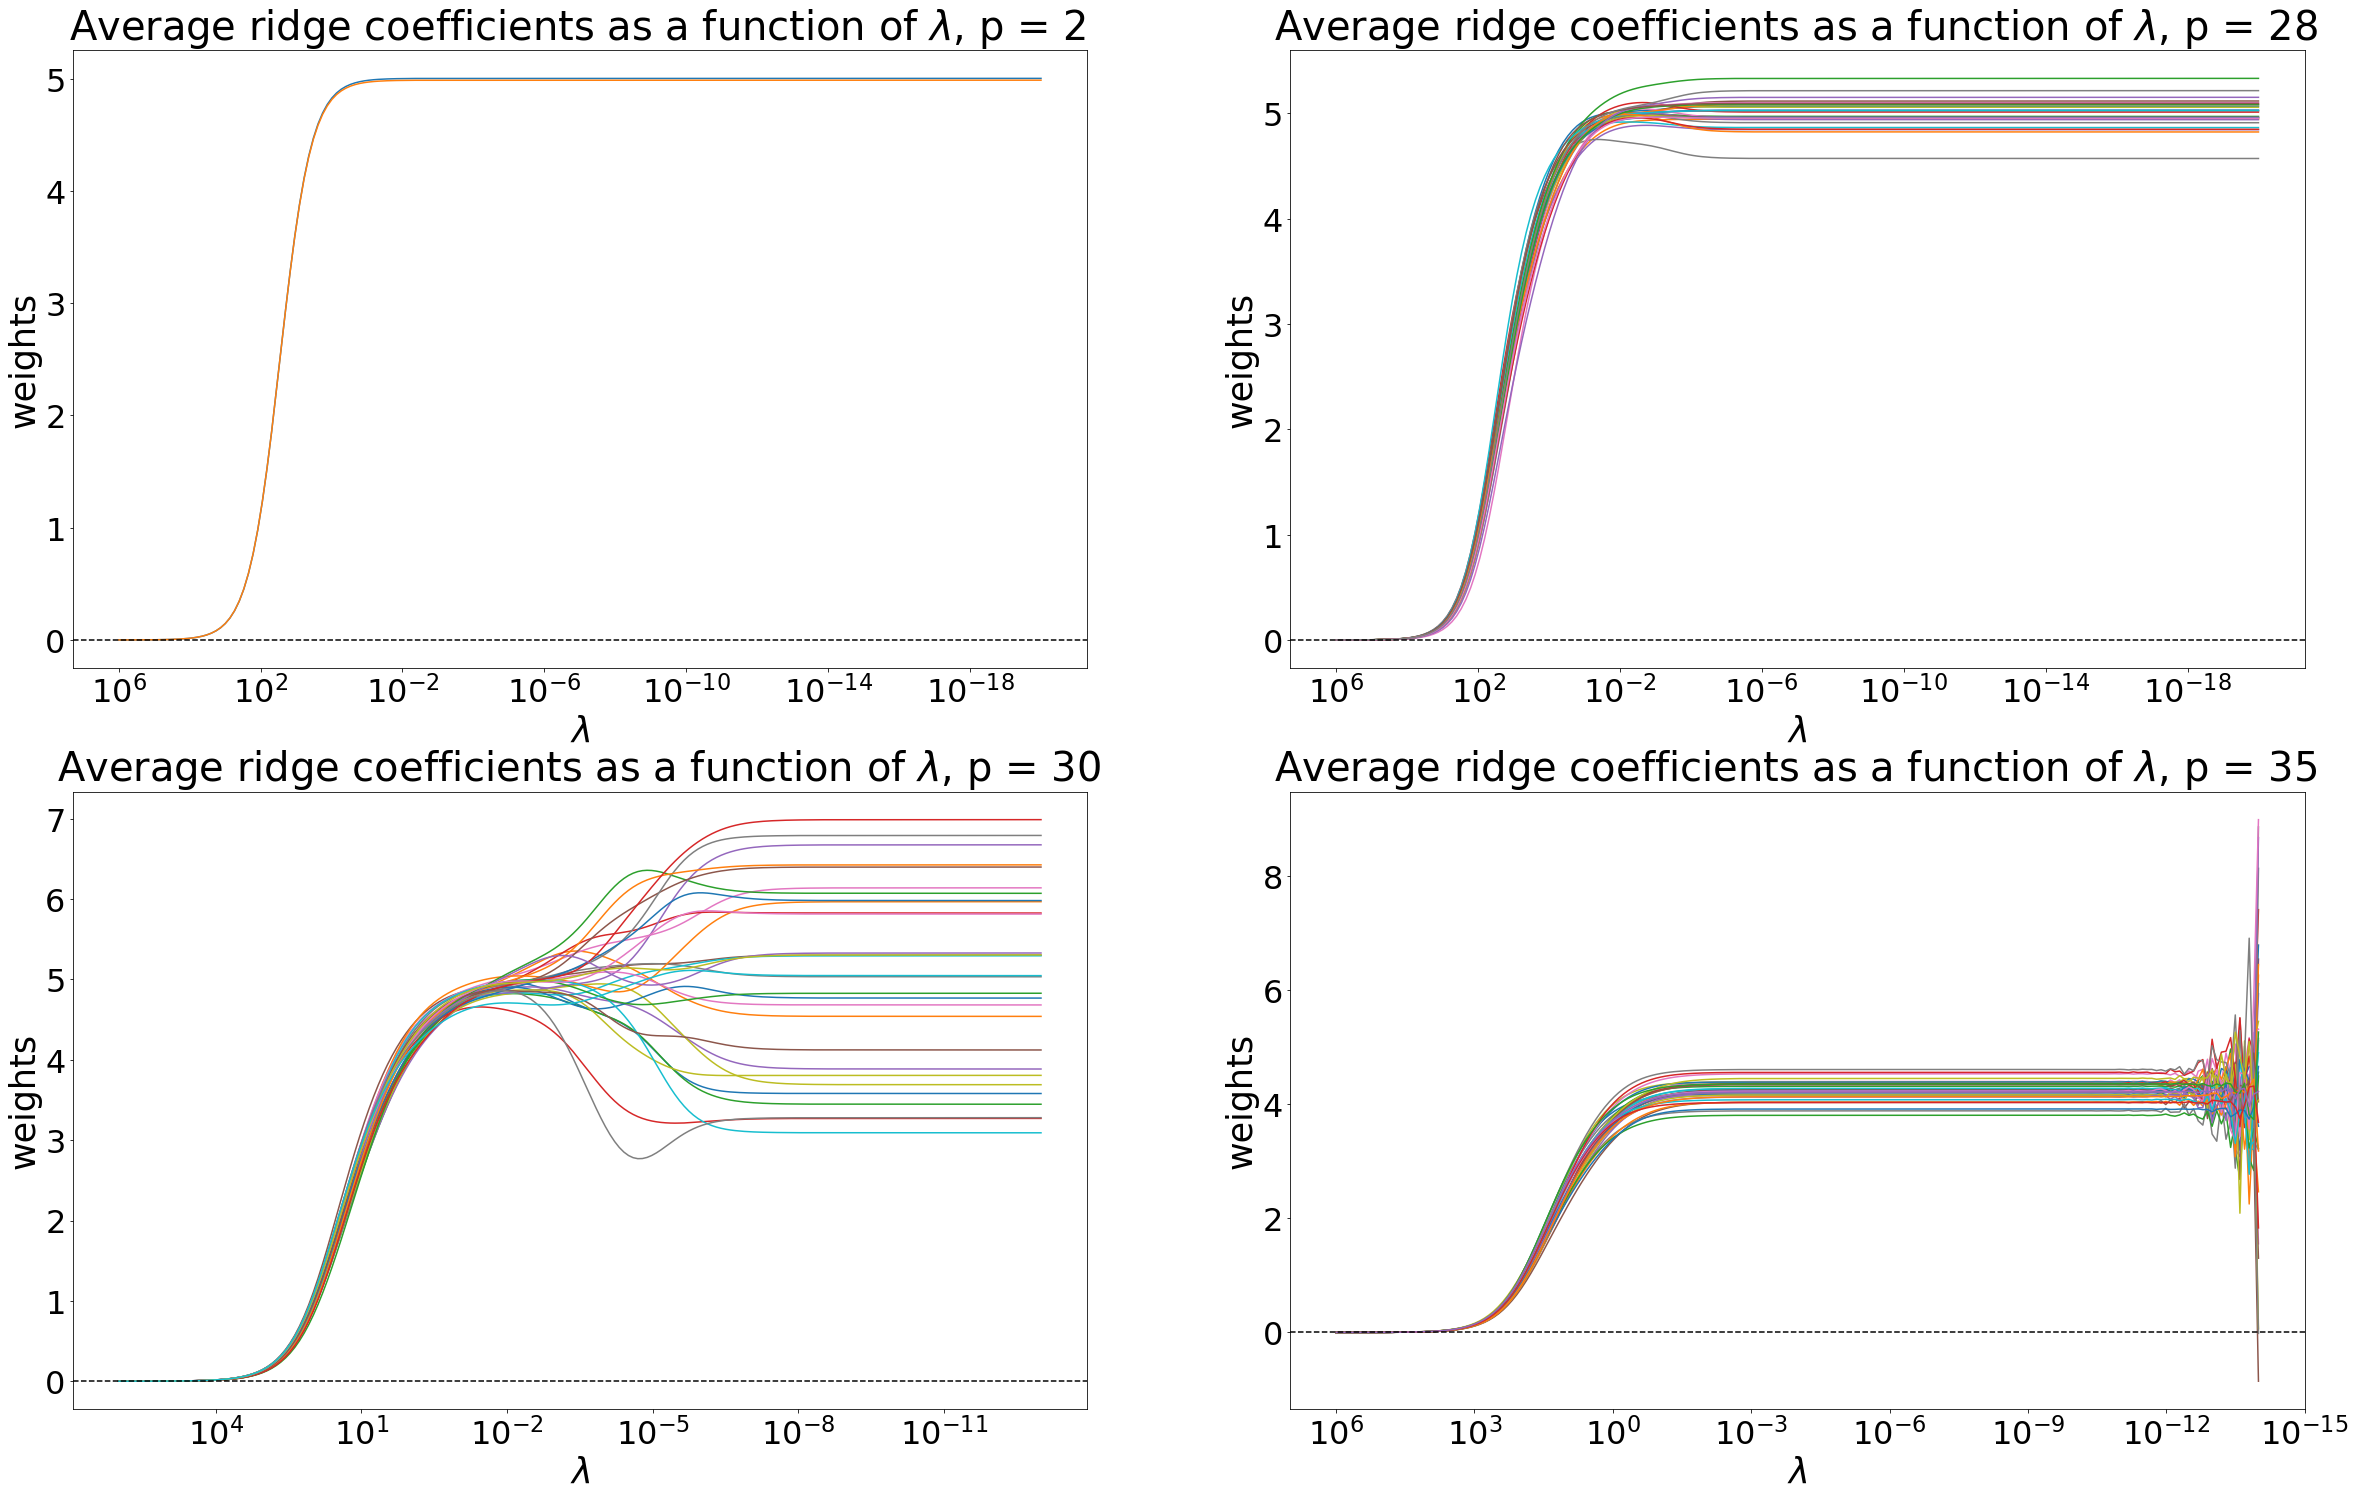
\includegraphics[scale=0.14]{Img/average_ridge_plot_betas.png}
        \centering
    \end{figure}
\end{frame}
%---------------------------------------------------------------------------%
\begin{frame}[fragile]
    \frametitle{Ridge Regression}
    Alternatively,
    \begin{align}
    \label{eqn:eqn2}
    \underset{\beta}{\operatorname{minimize}}\left\{\sum_{i=1}^{n}\left(y_{i}-\beta_{0}-\sum_{j=1}^{p} \beta_{j} x_{i j}\right)^{2}\right\} \text { subject to } \sum_{j=1}^{p}\beta_{j}^{2} \leq t,
    \end{align} \\
    where decreasing values of $t$ indicate an increasingly restrictive optimization constraint. \\
        %are equivalent to small values of $\lambda$.
    Ridge regression yields a closed-form solution for $\beta_{ridge}$:
        \begin{align}
        \label{eqn:eqn3}
        \hat{\beta}_{\lambda}^{R}=\mathbf{Z}_{\lambda} \hat{\beta}=\left(\mathbf{X}^{\prime} \mathbf{X} + \lambda \mathbf{I}\right)^{-1}\left(\mathbf{X}^{\prime} \mathbf{X}\right) \hat{\beta}
        \end{align}
    and for $var(\beta_{ridge})$:
        \begin{align}
        \label{eqn:eqn4}
        V\left(\hat{\boldsymbol{\beta}}_{\lambda}^{R}\right)=\sigma^{2}\left[\mathbf{X}^{\prime} \mathbf{X} + \lambda \mathbf{I}\right]^{-1}\left(\mathbf{X}^{\prime} \mathbf{X}\right)\left[\mathbf{X}^{\prime} \mathbf{X} + \lambda \mathbf{I}\right]^{-1}.
        \end{align}
\end{frame}
%---------------------------------------------------------------------------%
\begin{frame}[fragile]
    \begin{figure}[b]
        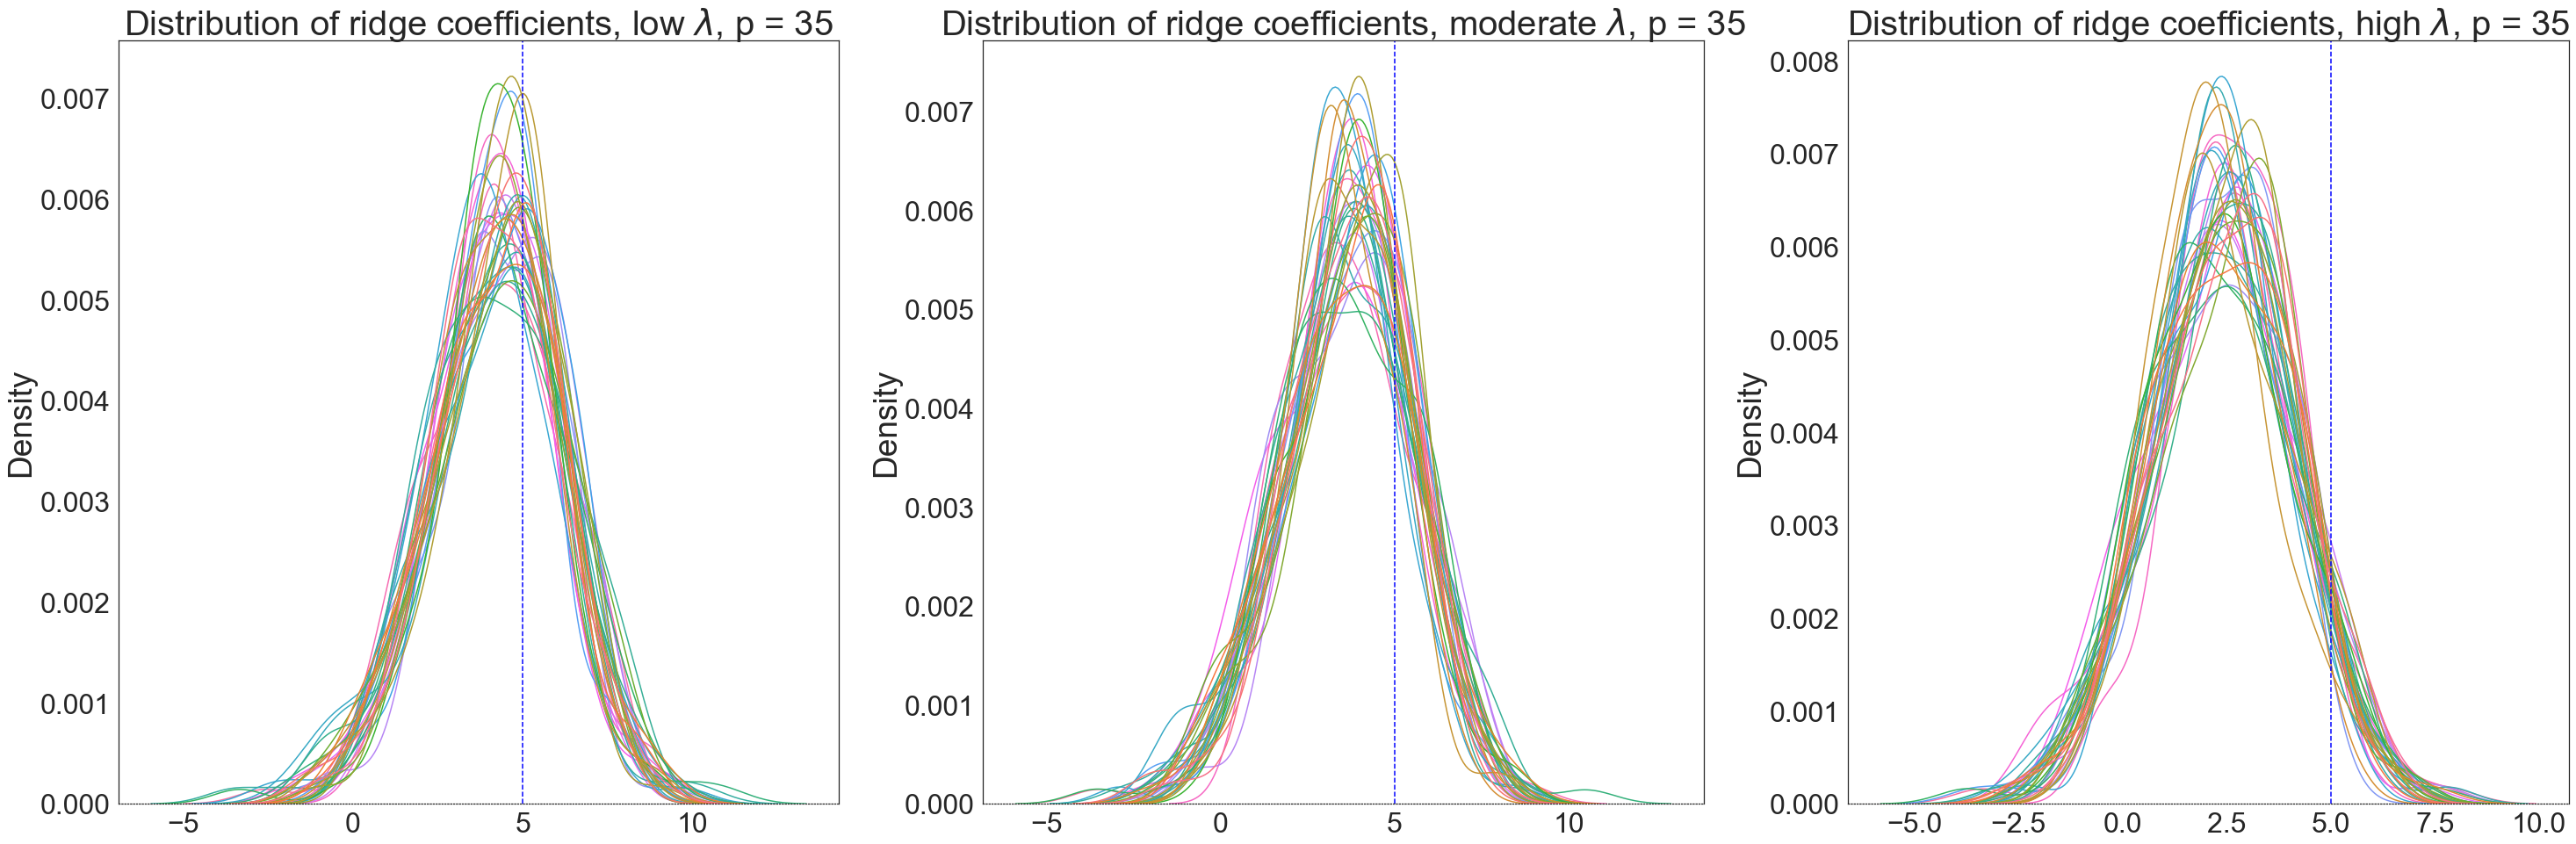
\includegraphics[scale=0.14]{Img/ridge_shrunken_beta_dist_35.png}
        \centering
    \end{figure}
\end{frame}
%---------------------------------------------------------------------------%
\begin{frame}[fragile]
    \frametitle{Lasso Regression}
    Consider the lasso minimization problem, which uses an $\ell_1$-norm constraint:
    \begin{align}
    \label{eqn:eqn5}
    \underset{\beta}{\operatorname{minimize}}\left\{\sum_{i=1}^{n}\left(y_{i}-\beta_{0}-\sum_{j=1}^{p} \beta_{j} x_{i j}\right)^{2}\right\} \text { subject to } \sum_{j=1}^{p}\left|\beta_{j}\right| \leq t,
    \end{align}
    \begin{itemize}
        \item where the $\hat{\beta}_{\lambda}^{L}$ solution is \textit{sparce}: the lasso model holds onto relevant (non-zero) coefficients and sets irrelevant coefficients to \textbf{zero} %(important when $p$ $>$ $n$).
        \item Unlike ridge, lasso is a quadratic programming problem that does not have a closed-form solution.
    \end{itemize}
\end{frame}
%---------------------------------------------------------------------------%
\begin{frame}[fragile]
        \begin{figure}[b]
        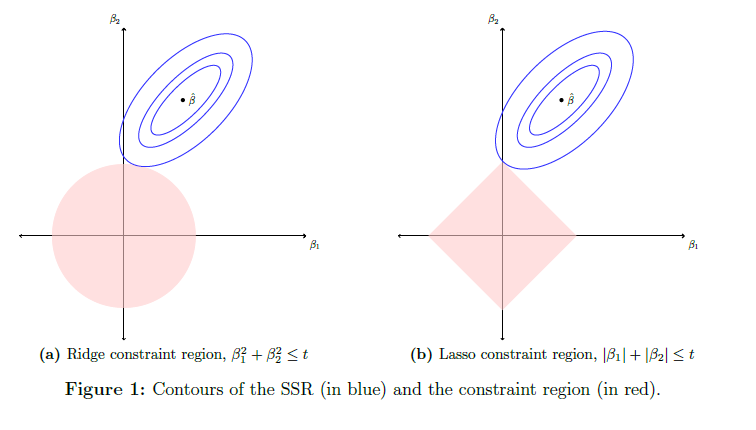
\includegraphics[scale=0.65]{Img/contours.png}\hspace{-1.2cm}
        \centering
    \end{figure}
\end{frame}
%---------------------------------------------------------------------------%
\begin{frame}[fragile]
    \frametitle{Lasso Regression}
    Limitations:
    \begin{itemize}
        \item Degree of sparsity
        \begin{itemize}
            \item Lasso does poorly when a large subset of regressors are $\{j:\beta_j \neq 0\}$ of $\{1,...,p\}$ 
        \end{itemize}
        %\item In the case of grouped multicollinearity, lasso will only select one variable from the group.
            %\begin{itemize}
                %\item Omitted variable bias.
            %\end{itemize}
        \item With high pairwise correlation among predictors, ridge regression outperforms lasso in terms of prediction.
        \item Lasso can only select up to $n$ regressors when $p$ > $n$.
    \end{itemize}
\end{frame}
%---------------------------------------------------------------------------%
\begin{frame}[fragile]
    \begin{figure}[b]
        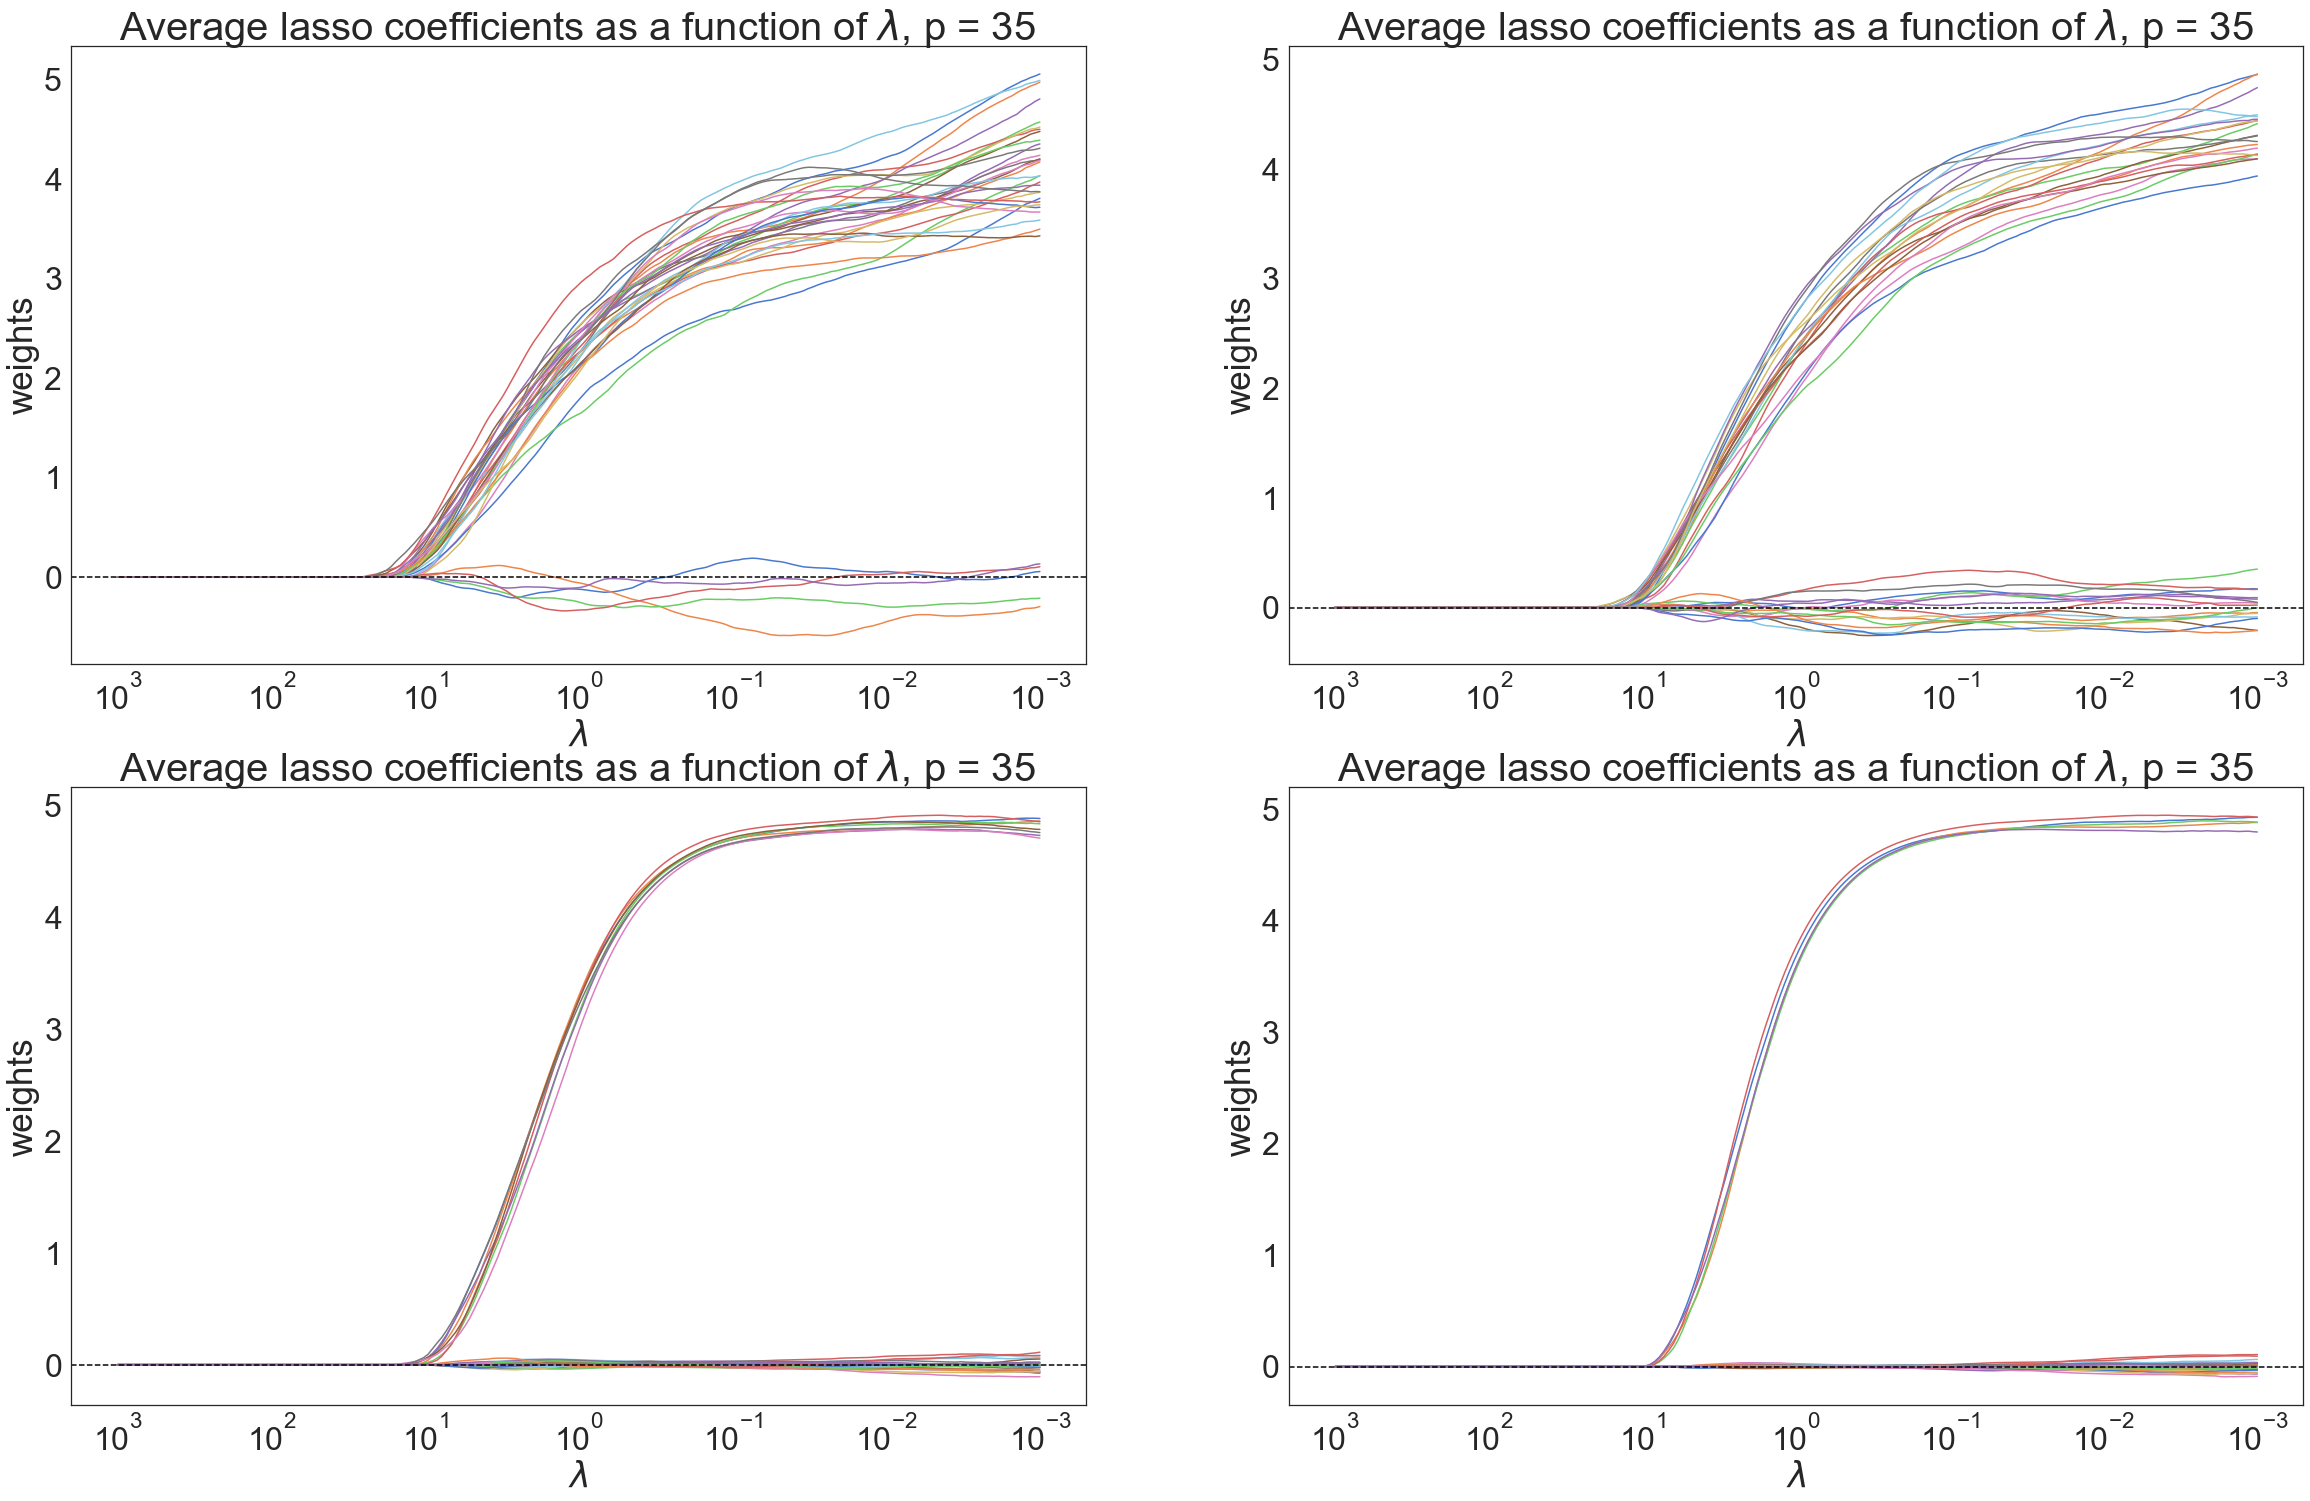
\includegraphics[scale=0.14]{Img/average_lasso_plot_betas.png}
        \centering
    \end{figure}
\end{frame}
%---------------------------------------------------------------------------%
\begin{frame}[fragile]
%\frametitle{Variance-Bias Tradeoff}
    \begin{figure}[b]
        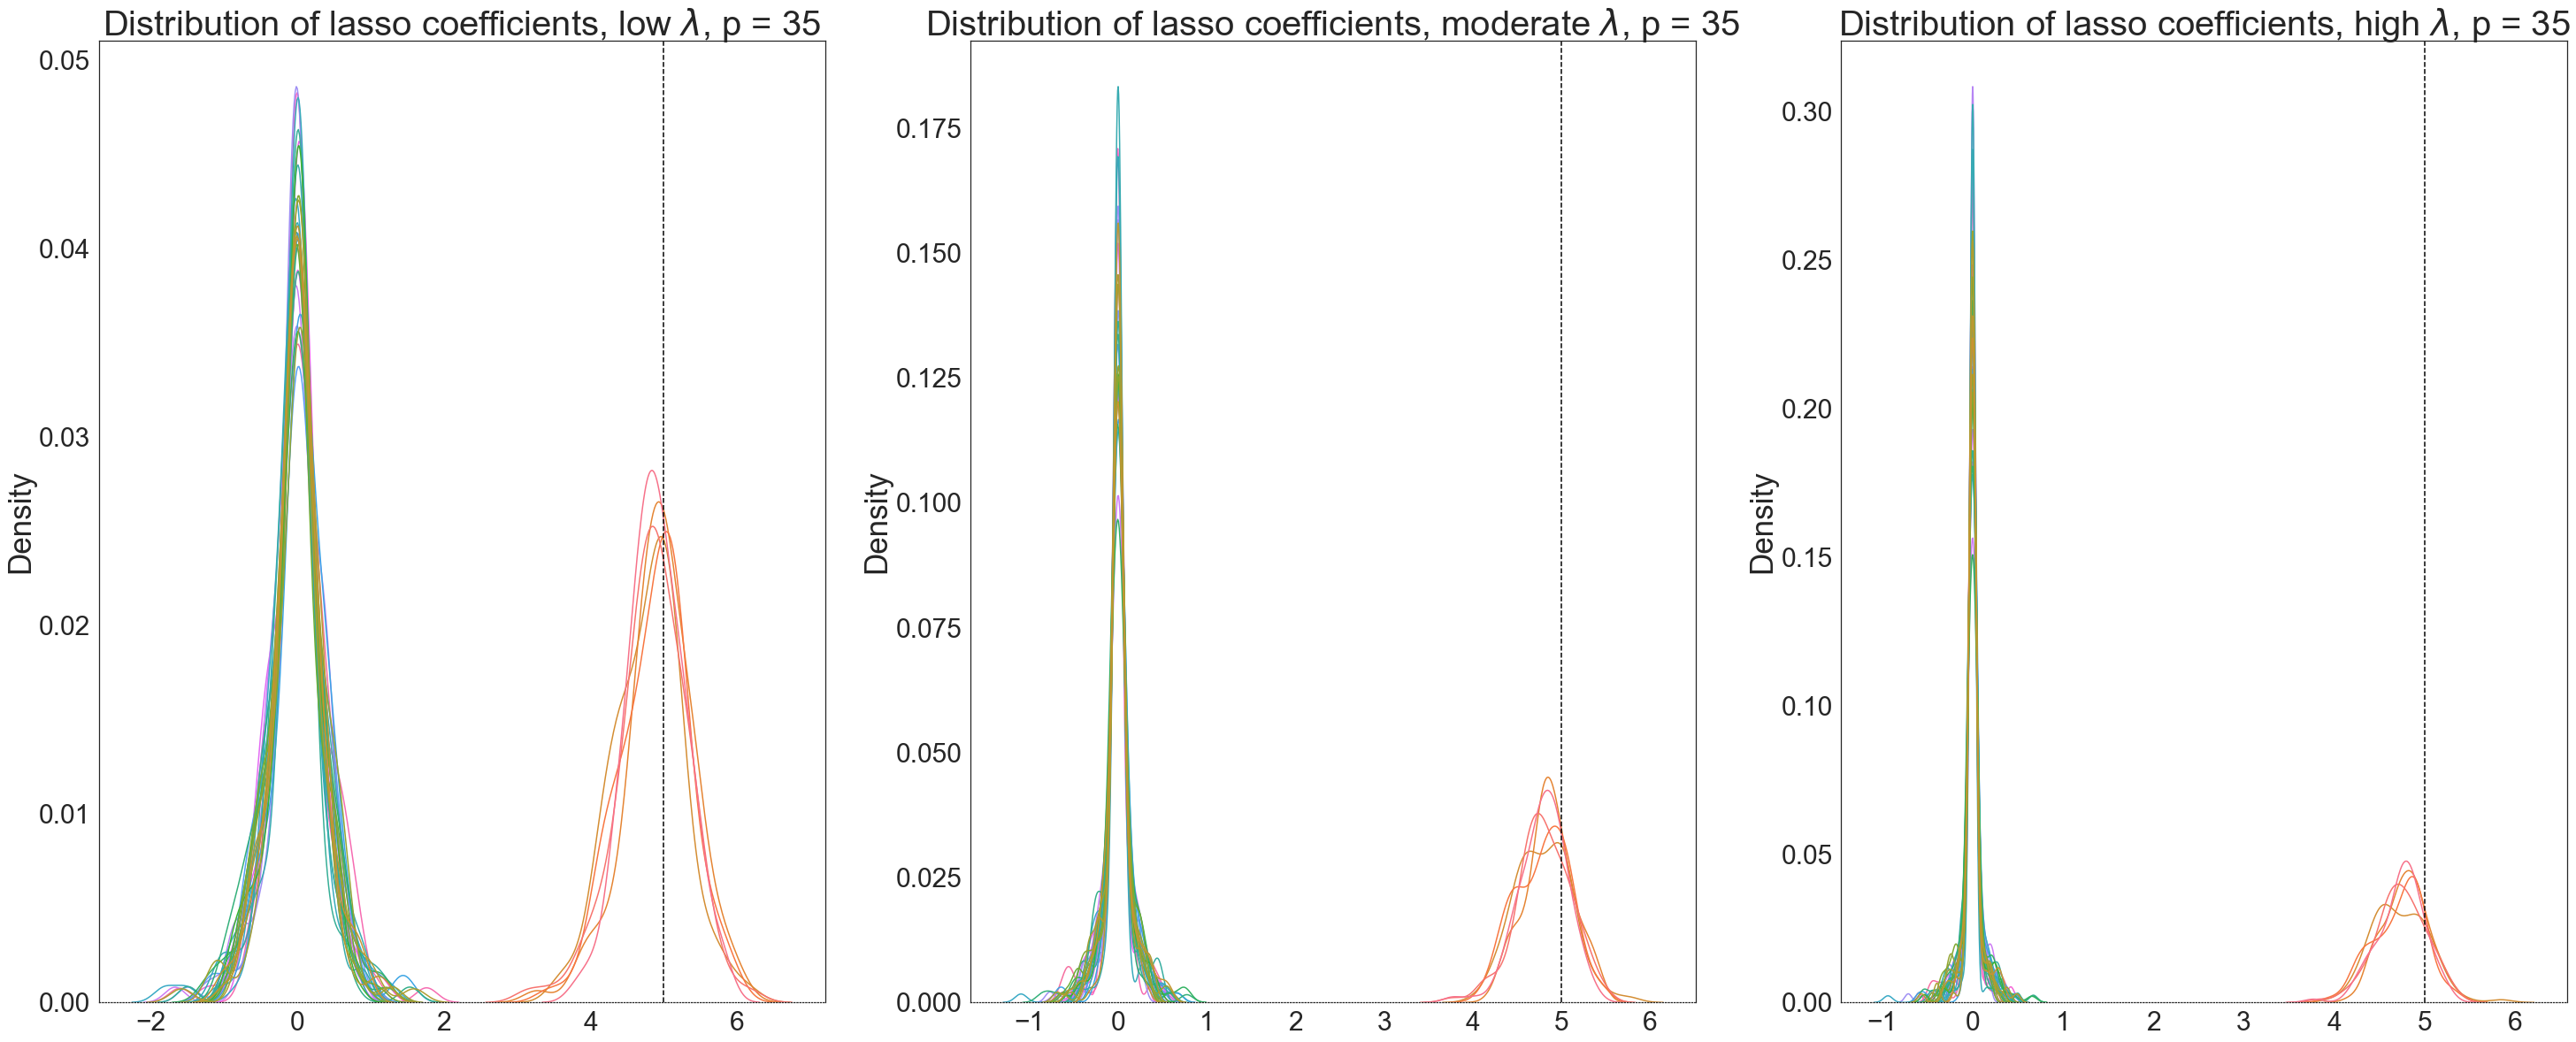
\includegraphics[scale=0.15]{Img/lasso_shrunken_beta_dist_35.png}
        \centering
    \end{figure}
\end{frame}
%---------------------------------------------------------------------------%
\begin{frame}[fragile]
    \frametitle{"Naïve" Elastic Net Regression}
    Consider the "naïve" elastic net minimization problem, which is subject to a constraint that is represented as a convex combination of the ridge and lasso shrinkage penalties:
    \begin{align}
    \label{eqn:eqn6}
    \underset{\beta}{\operatorname{minimize}}\left\{\sum_{i=1}^{n}\left(y_{i}-\beta_{0}-\sum_{j=1}^{p} \beta_{j} x_{i j}\right)^{2}\right\} \text { subject to } \left(1 - \alpha \right)\sum_{j=1}^{p}\left|\beta_{j}\right| + \alpha \sum_{j=1}^{p}\beta_{j}^{2} \leq t
    \end{align}
    where $\alpha$ represents the weight assigned to the ridge penalty. 
    %where $\alpha = \lambda_{2} / \left(\lambda_{1} + \lambda_{2}\right)$ .
    \begin{itemize}
        \item Contains the best features of ridge and lasso regression (continuous shrinkage and simultaneous variable selection).
        \begin{itemize}
            \item For all $\alpha \in [0, 1)$, the elastic net penalty function is singular at 0 and strictly convex for all $\alpha > 0$.
            \item Strict convexity is what sets elastic net apart from lasso.
        \end{itemize}
    \end{itemize}
\end{frame}
%---------------------------------------------------------------------------%
\begin{frame}[fragile]
    \frametitle{"Naïve" Elastic Net Regression}
    \begin{itemize}
        \item \textbf{Improves over the lasso by}
            \begin{itemize}
                \item overcoming the saturation of variable selection when $p > n$. \textbf{(variable selection)}
                \item accounting for highly correlated "grouped" variables. \textbf{(continuous shrinkage)}
                \item strengthening prediction performance if substantial multicollinearity among predictors exists in cases where $n > p$.
            \end{itemize}
        %\item Intuition: for each fixed $\lambda$ we find ridge coefficients and then lasso coefficients.
        \item \textbf{Limitations}
            \begin{itemize}
                \item Double shrinkage does not reduce variance and unnecessarily introduces added bias.
                \item Hence, works only when its solution is very close to either ridge or lasso.
            \end{itemize}
    \end{itemize}
\end{frame}
%---------------------------------------------------------------------------%
\begin{frame}[fragile]
    \frametitle{Elastic Net Regression}
    Given the data set (y,X) and the two fixed non-zero Lagrangian parameters, ($\lambda_{1}$,$\lambda_{2}$), derived from the naïve elastic net's optimization problem, \emph{Lemma 1} of \cite{zou2005regularization} defines the artificial data set ($\mathbf{y}^*$, $\mathbf{X}^*$): 
    
    \begin{align}
        \label{eqn:eqn7}
            \hat{\beta}^*=\arg \min_{\hat{\beta}^*}|\mathbf{y}^* - \mathbf{X}^*\beta^*|^2 + \frac{\lambda_1}{\sqrt{(1+\lambda_2)}}|\beta^*|_{1}
    \end{align}
    
    With the corrected elastic net estimates $\hat{\beta}$ defined as 
    \begin{align}
        %\label{eqn:eqn8}
            \hat{\beta}(elastic \: net)=\sqrt{(1+\lambda_2)}\hat{\beta^*}
    \end{align}
    and 
    \begin{align}
        %\label{eqn:eqn9}
            \hat{\beta}(naive \: elastic \: net)={1 / \sqrt{(1+\lambda_2)}}\hat{\beta^*}
    \end{align}
    
    Finally,
    \begin{align}
        \label{eqn:eqn10}
            \hat{\beta}(elastic \: net)=(1+\lambda_2)\hat{\beta}(naive \: elastic \: net). 
    \end{align}
\end{frame}
%---------------------------------------------------------------------------%
\begin{frame}[fragile]
    \begin{figure}[b]
        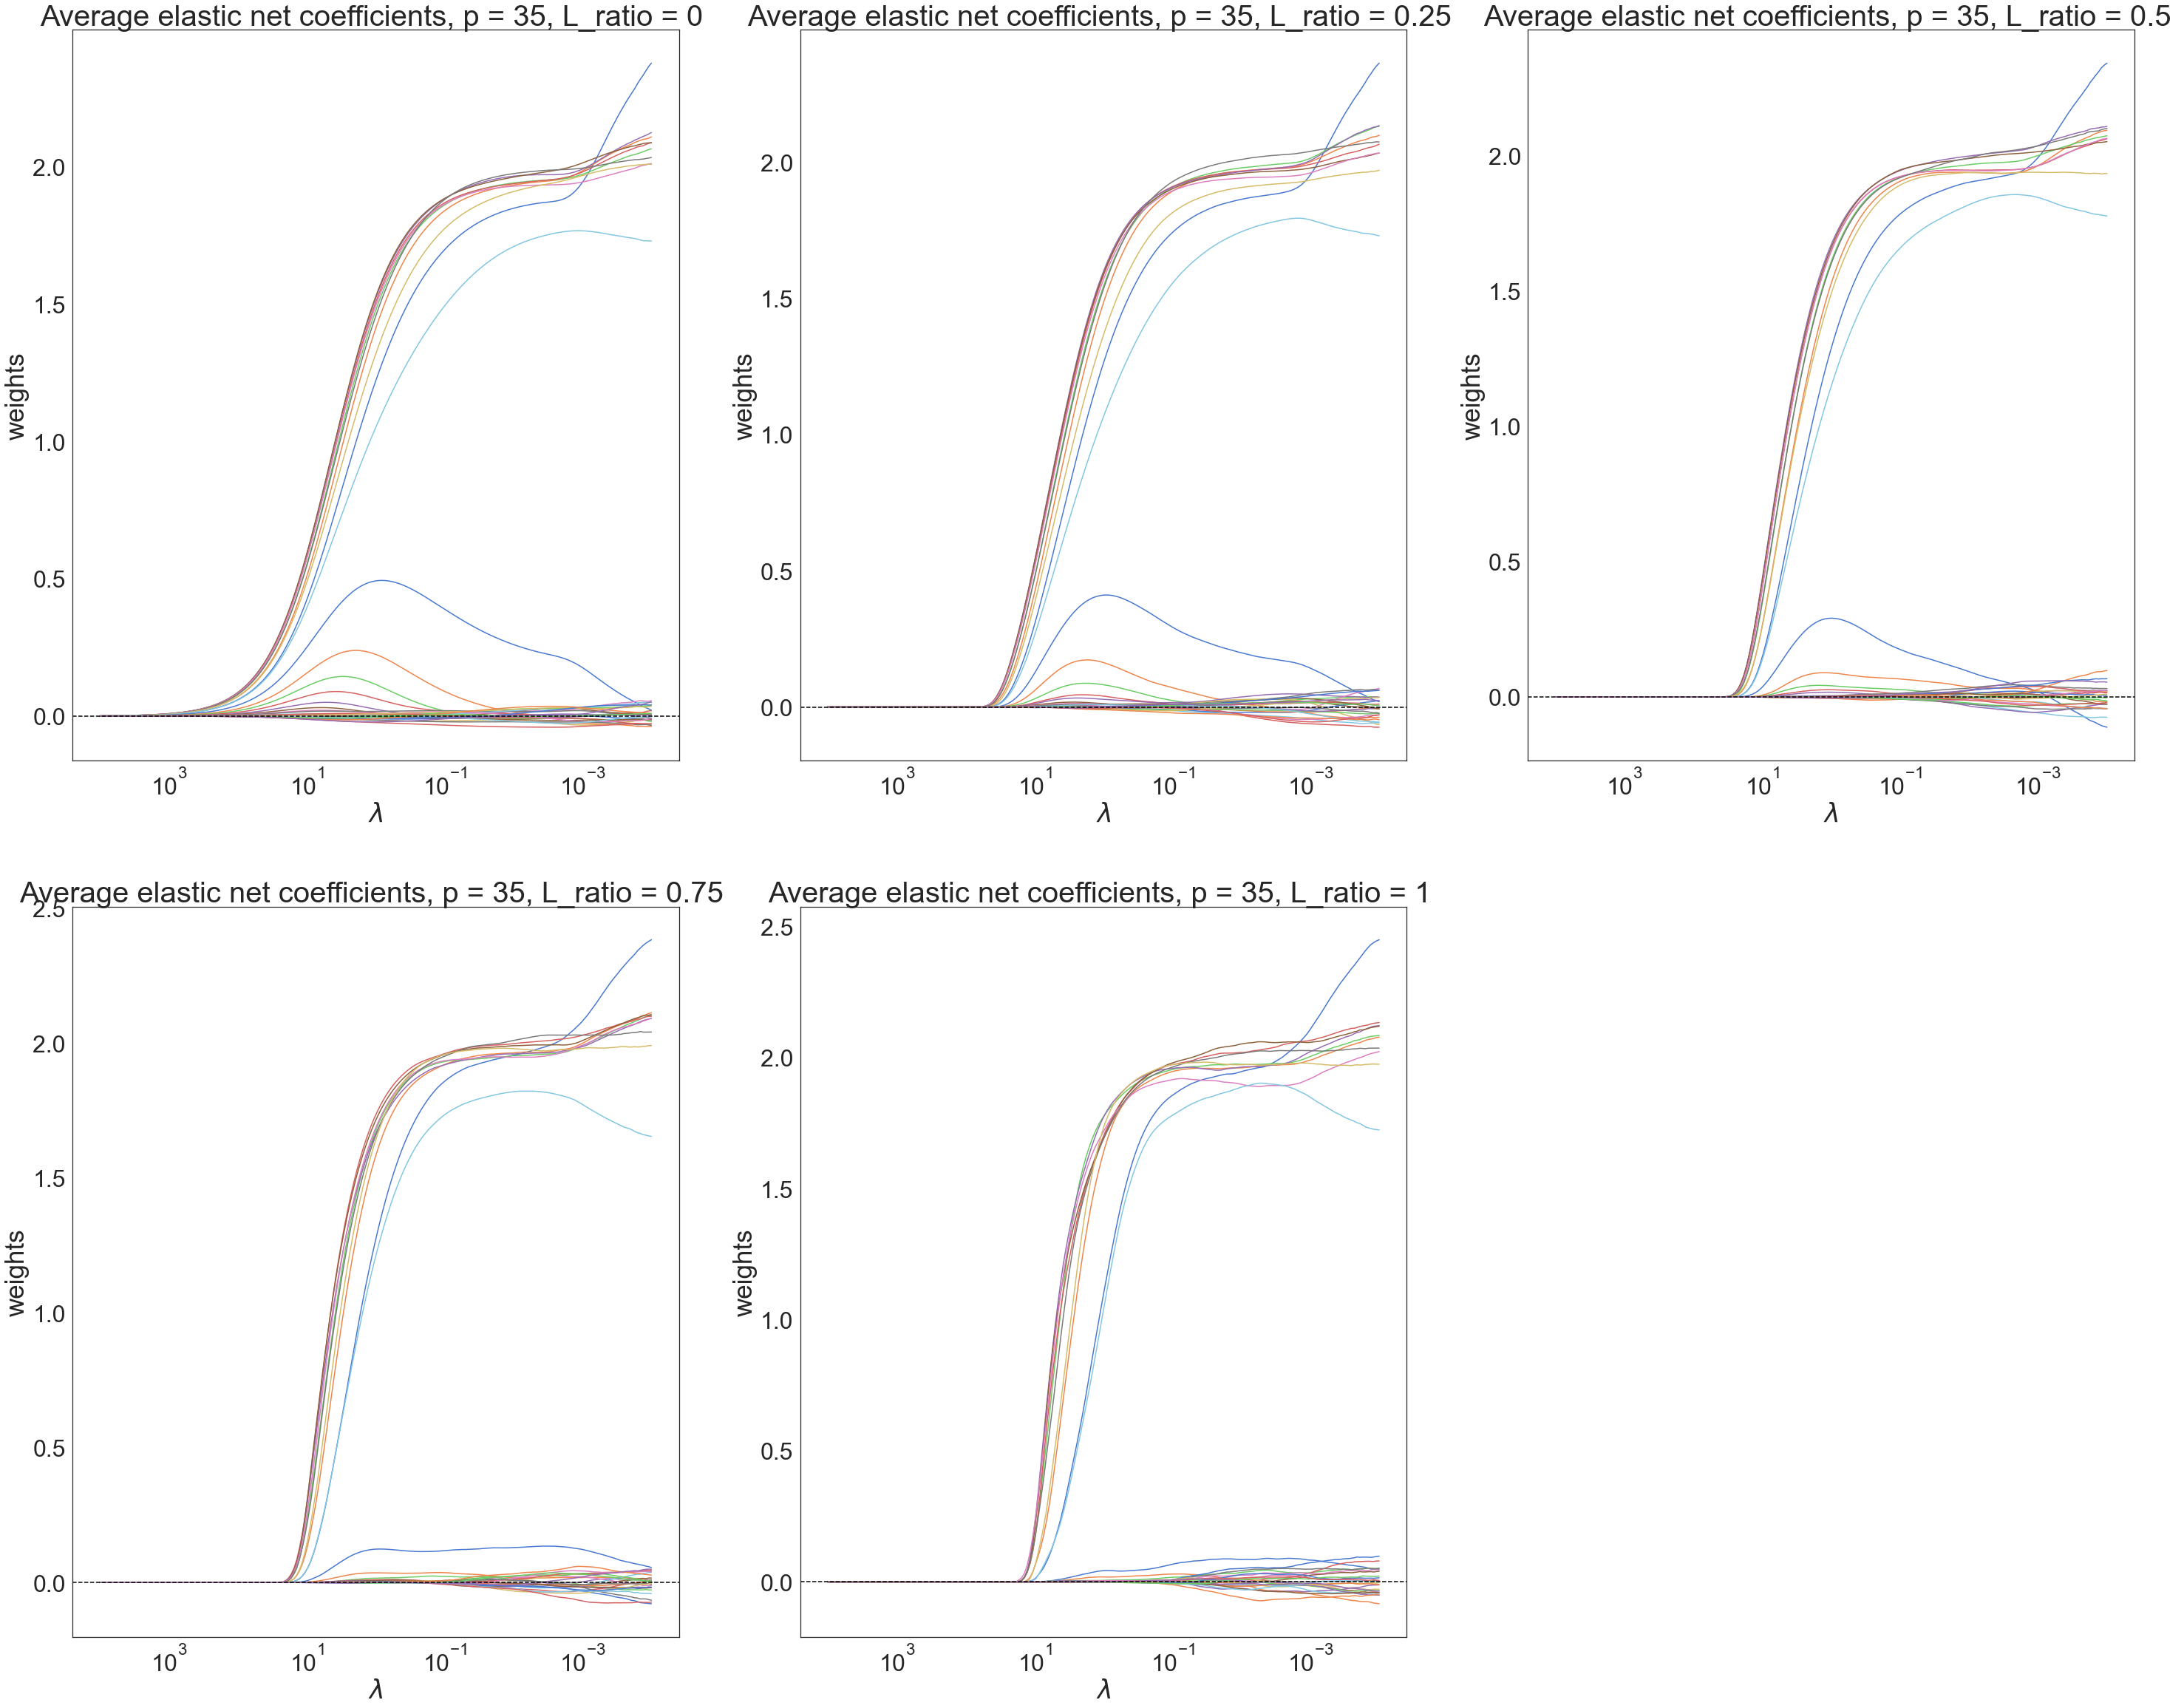
\includegraphics[scale=0.095]{Img/elastic_net_plot_average_betas.png}
        \centering
    \end{figure}
\end{frame}
%---------------------------------------------------------------------------%
\begin{frame}[fragile]
    \begin{figure}[b]
        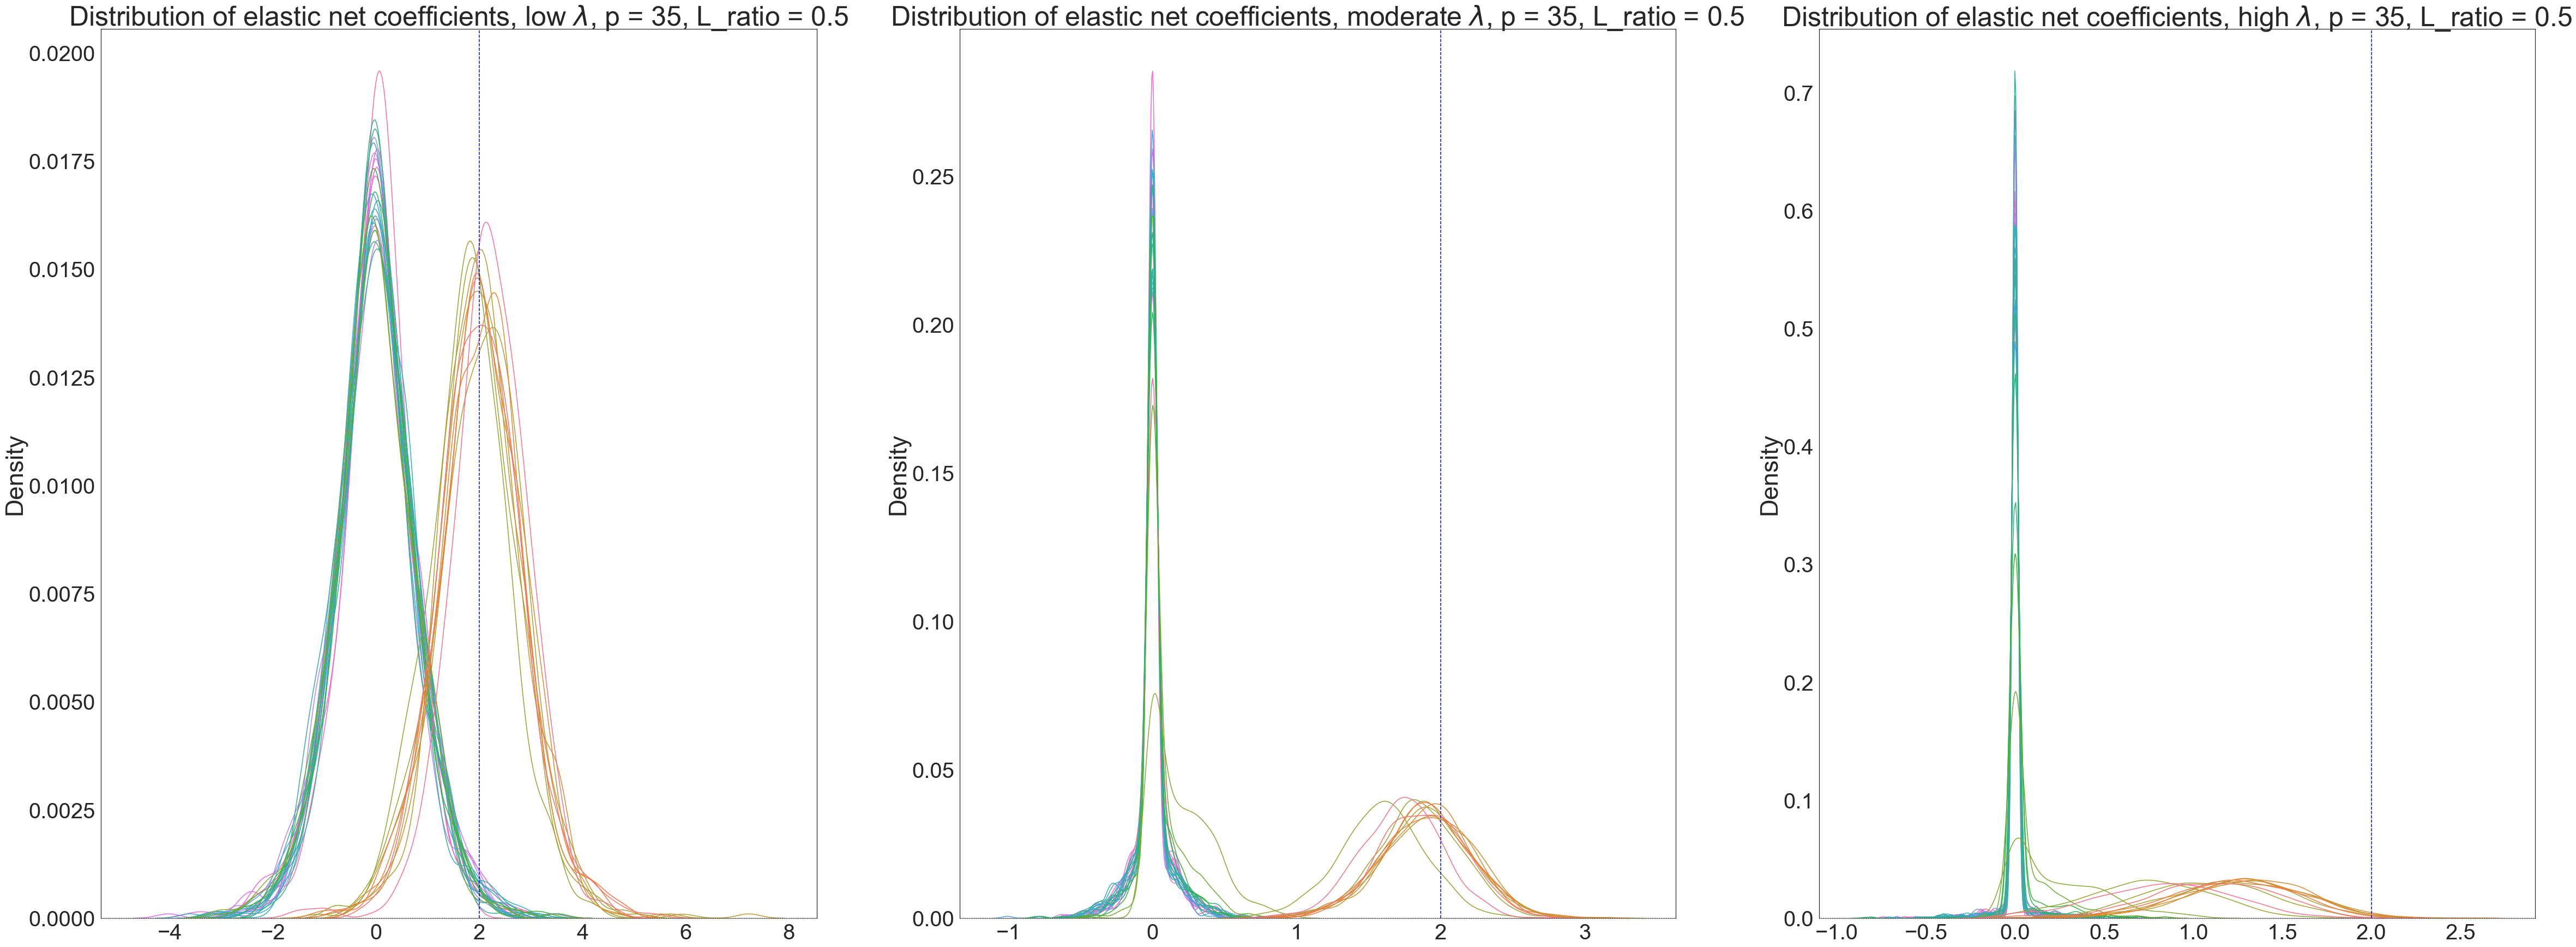
\includegraphics[scale=0.09]{Img/elastic_net_shrunken_beta_dist_35_0.5.png}
        \centering
    \end{figure}
\end{frame}
%---------------------------------------------------------------------------%
\begin{frame}[fragile]
\frametitle{Regularization Methods Summarized}
\tiny
\begin{table}
\begin{tabular}[h]{ ||m{2cm}|m{5cm}|m{5cm}||  }
\hline
Model & Characteristics & Drawbacks \\
\hline\hline
Ridge
& 
\begin{itemize}
    \item $\ell_2$-norm shrinkage penalty %($\hat{\beta} \rightarrow 0$)
    \item Performs well in the presence of multicollinearity.
\end{itemize}
& 
\begin{itemize}
    \item Does not perform variable selection.
\end{itemize} \\
\hline
Lasso
& 
\begin{itemize}
    \item  $\ell_1$-norm shrinkage penalty %($\hat{\beta} = 0$)
    \item Performs variable selection.
\end{itemize}
& 
\begin{itemize}
    \item Does not behave well when sparsity is very low.
    \item Cannot handle high correlation or grouped multicollinearity. 
    \item Can only select up to $n$ regressors when $p > n$
\end{itemize} \\
\hline
Naïve Elastic Net
& 
\begin{itemize}
    \item  convex combination of $\ell_1$-norm and $\ell_2$-norm shrinkage penalties. 
    \item Potentially selects all $p$ in the presence of grouped collinearity.
\end{itemize}
& 
\begin{itemize}
    \item Double shrinkage does not contribute to further reduction of the variances and adds unnecessary bias.
    \item Works only when solution is very close to ridge or lasso.
\end{itemize} \\
\hline
Elastic Net
&
\begin{itemize}
    \item Maintains all characteristics from naïve model, but corrects for double shrinkage.
\end{itemize}
&
\tabularnewline
\hline
\end{tabular}
% \caption{Summary of methodologies}
% \label{table:1}
\end{table}
\end{frame}
%---------------------------------------------------------------------------%
%\begin{frame}
%\begin{columns}[t]
%\column{.5\textwidth}
%\centering
%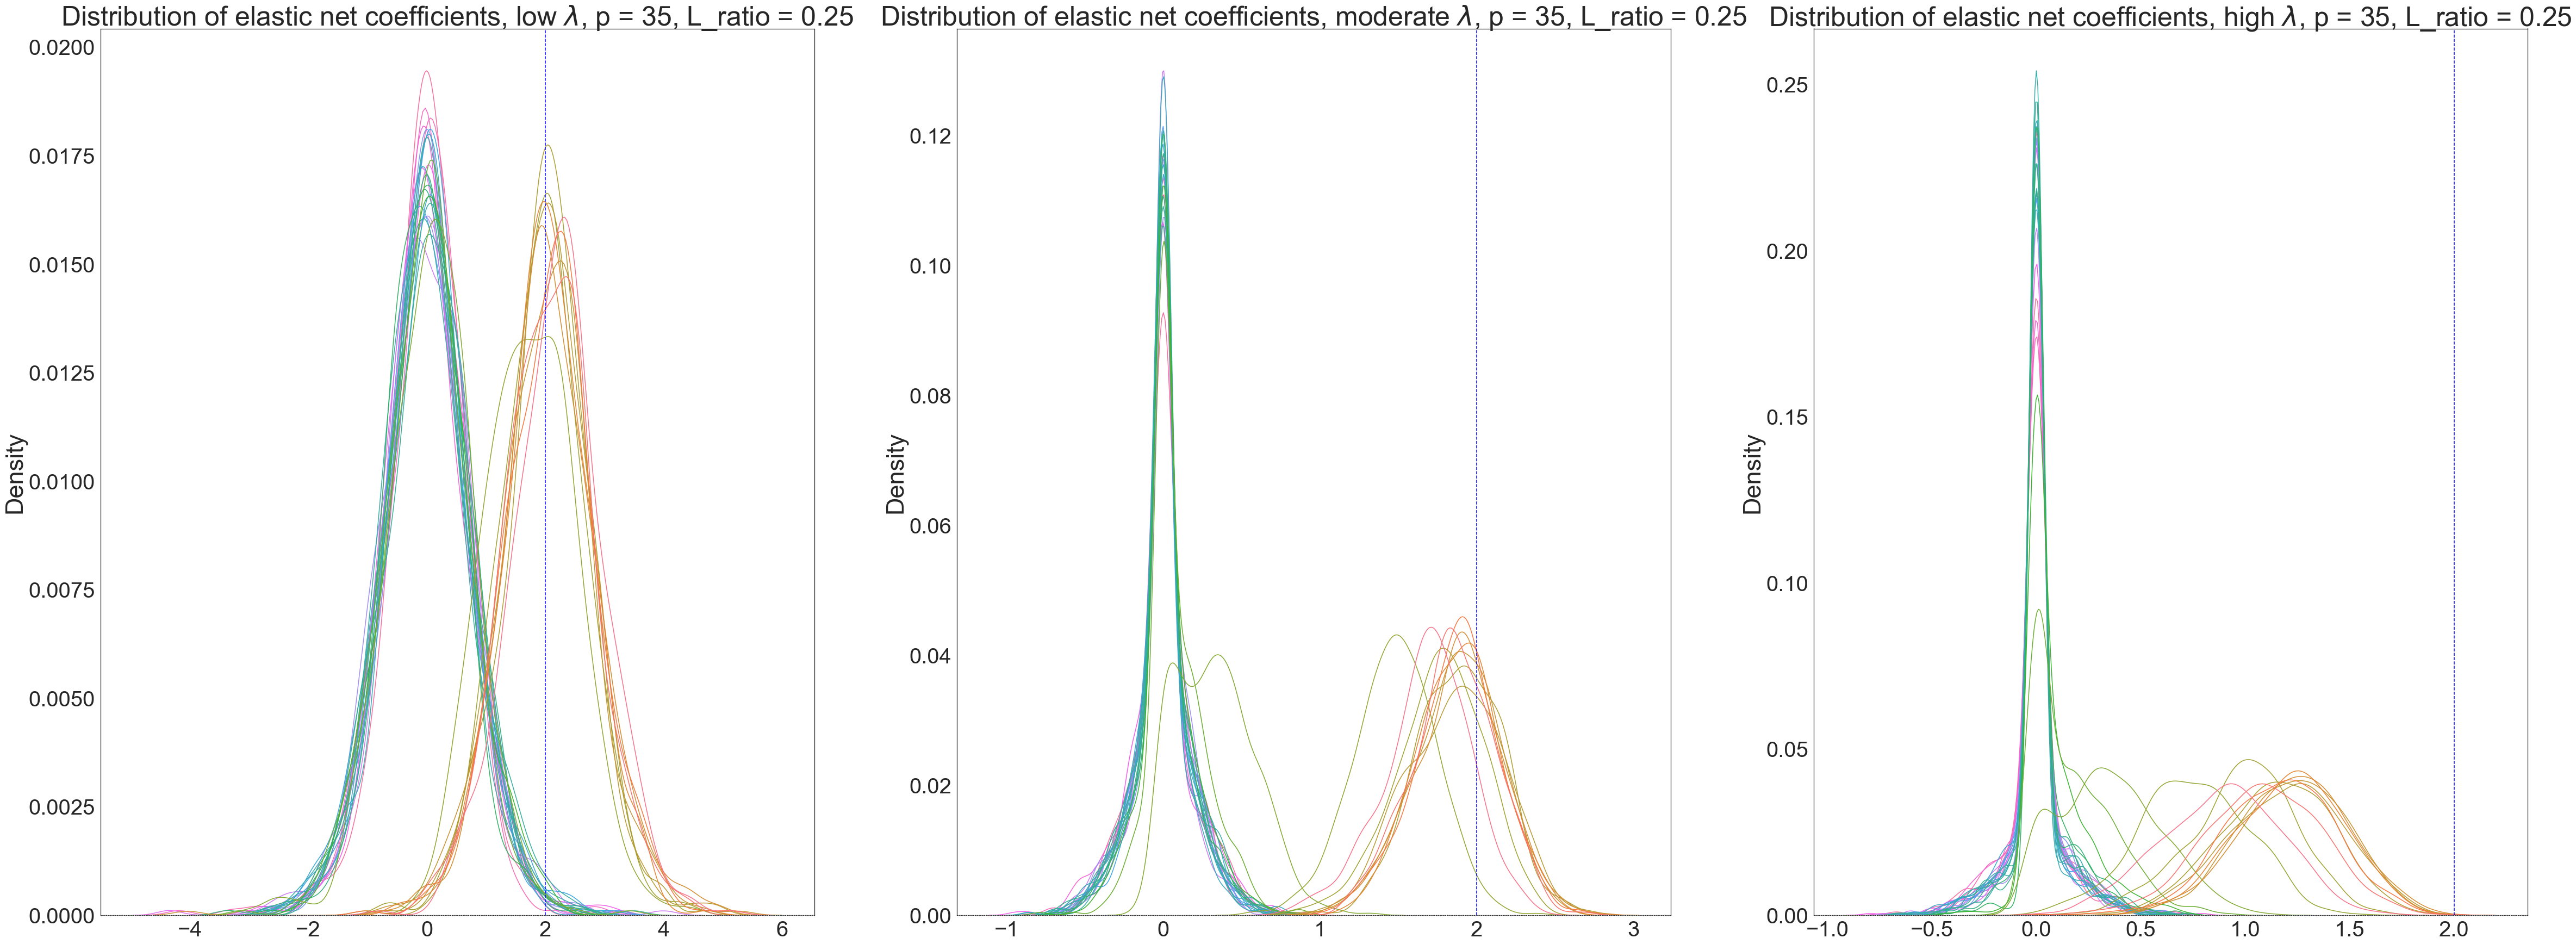
\includegraphics[width=7cm,height=4cm, left]{Img/elastic_net_shrunken_beta_dist_35_0.25.png}
%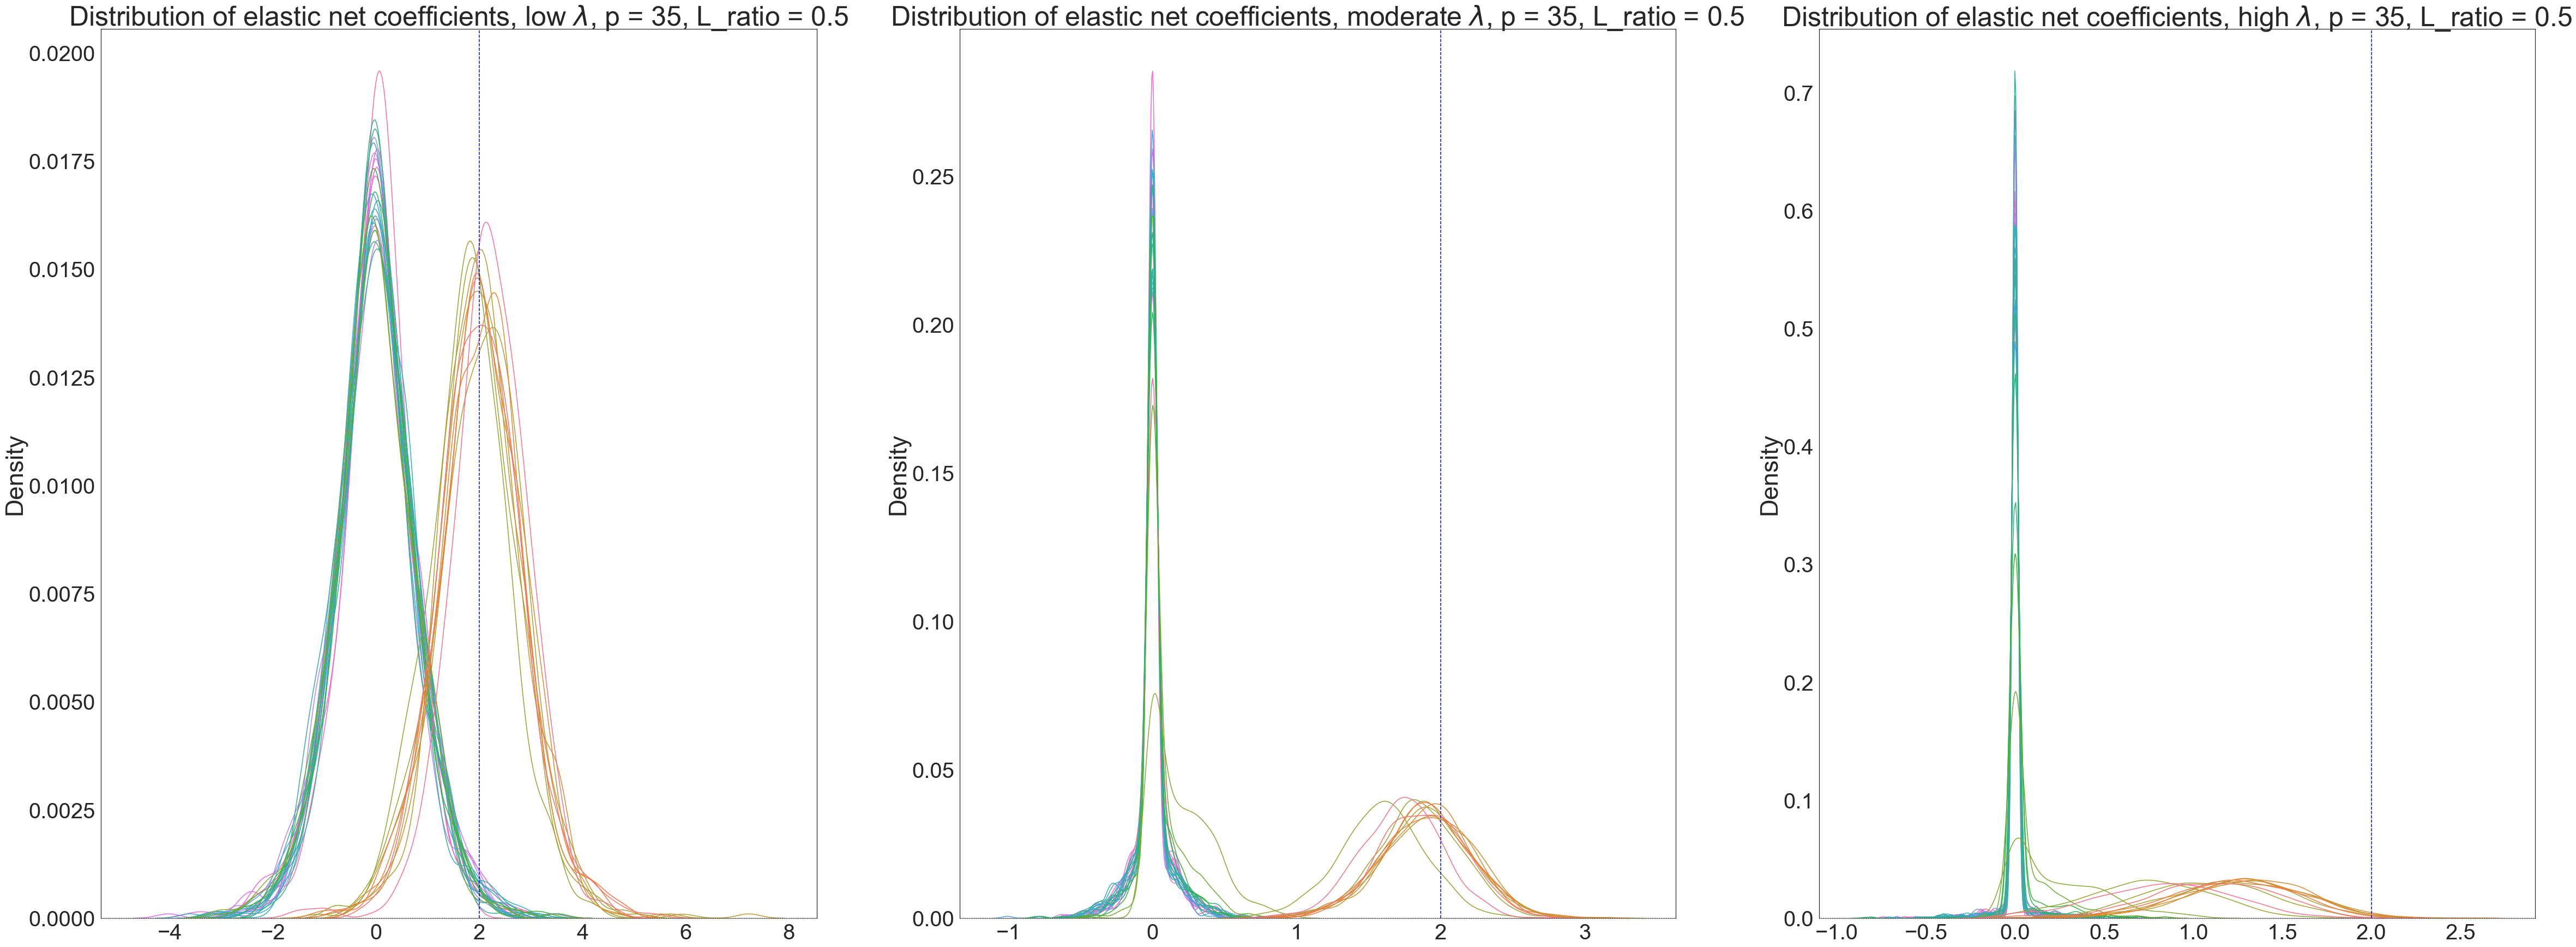
\includegraphics[width=7cm,height=4cm, right]{Img/elastic_net_shrunken_beta_dist_35_0.5.png}\\
%\column{1.0\textwidth}
%\centering
%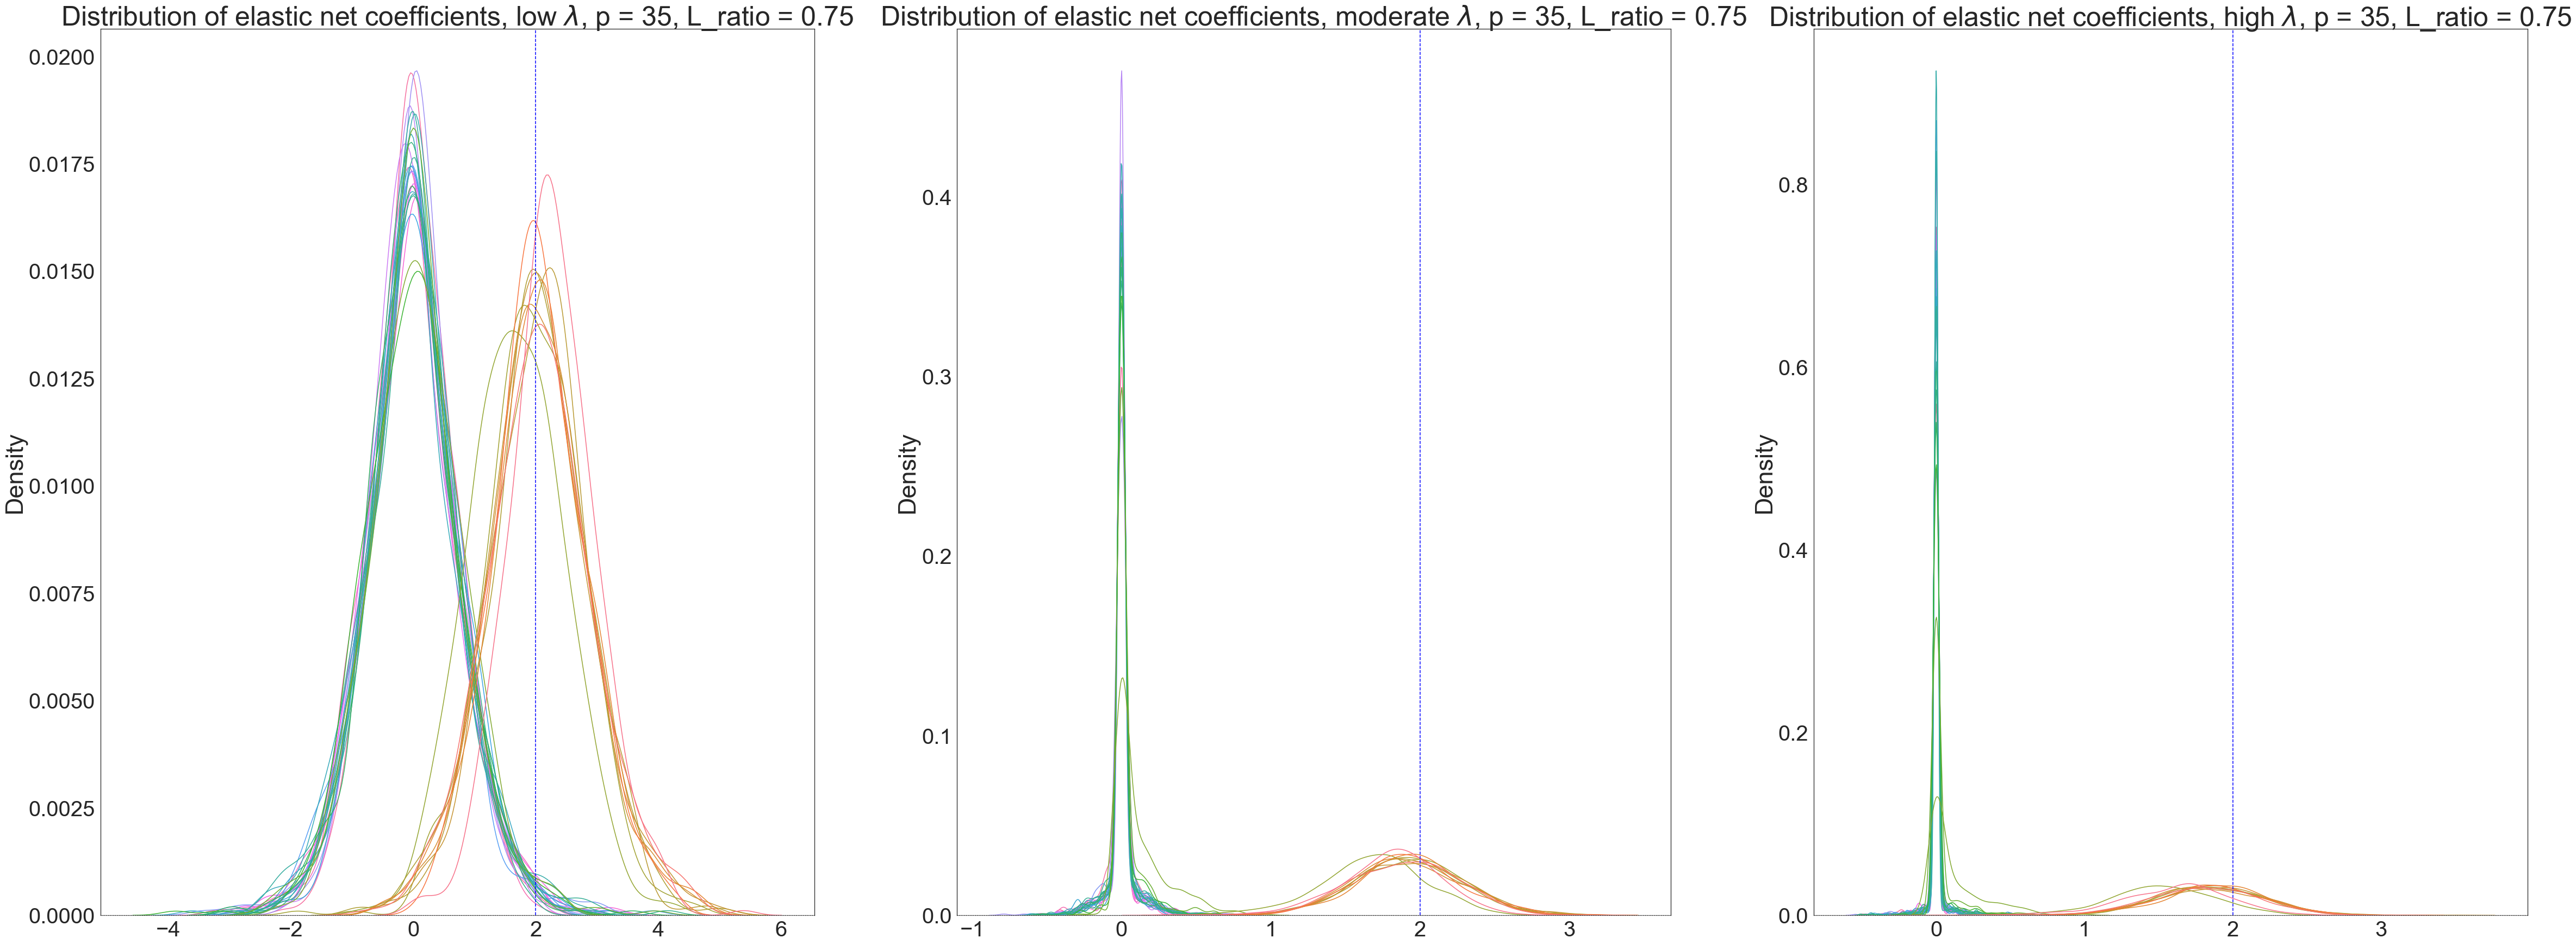
\includegraphics[width=7cm,height=4cm, center]{Img/elastic_net_shrunken_beta_dist_35_0.75.png}\\
%\end{columns}
%\end{frame}